% Draft figure environments for author review; main.tex does not include them yet.
% Compile with the manuscript directory as the working directory.

\begin{figure*}[t]
  \centering
  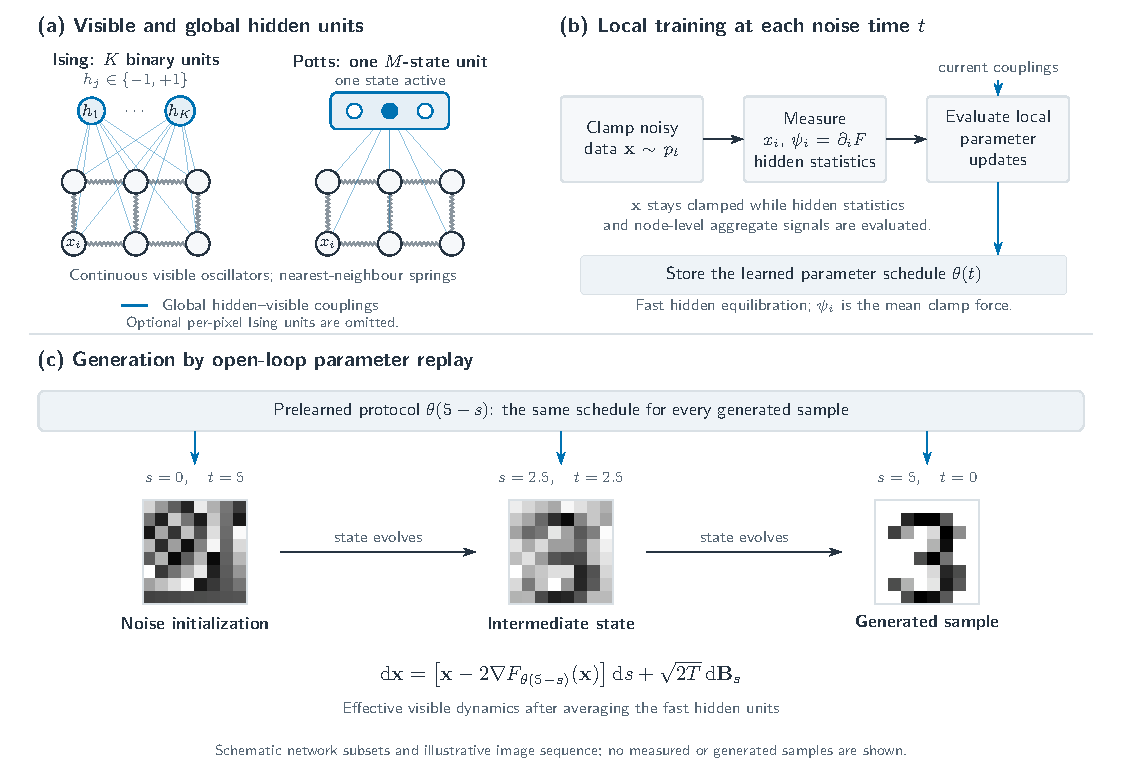
\includegraphics[width=\textwidth]{figures/conceptual_draft.pdf}
  \caption{\textbf{Local learning and open-loop generation with hidden degrees of freedom.}
  (a) Continuous visible oscillators with neighbour springs couple globally to
  either $K$ Ising units or one Potts unit with $M$ mutually exclusive states.
  Representative network subsets are shown; optional per-pixel Ising units
  are omitted. (b) At each noise time, visible units are clamped to noisy data.
  Mean clamp forces, conditional hidden statistics, node-level aggregate
  signals and current couplings determine local parameter updates.
  (c) The timeline indicates progression through the learned parameter
  schedule, represented by the same schematic curve icon as in (b).
  Frame spacing is schematic. The prescribed schedule is shared across samples.
  Images show one real reverse-SDE trajectory from the trained
  $28\times28$ four-digit (0, 1, 2, 3) model, with 784 states in the global
  Potts unit and 784 per-pixel Ising units. Trajectory index 0 of the original
  500-sample base set (seed 2026) was fixed before viewing. The displayed
  five states are recorded near generation times $s=0,2.5,4,4.5,5$; they are not blended
  images. All frames use the same pixel-intensity scale, clipped to $[0,1]$
  and shown as white digits on black. Sampling uses the effective visible
  dynamics in the fast-hidden-equilibration limit. Panels (a,b) and the
  schedule icon are schematic; the full sampling and frame provenance are
  retained with the figure data.}
  \label{fig:latent_conceptual_draft}
\end{figure*}

\begin{figure*}[t]
  \centering
  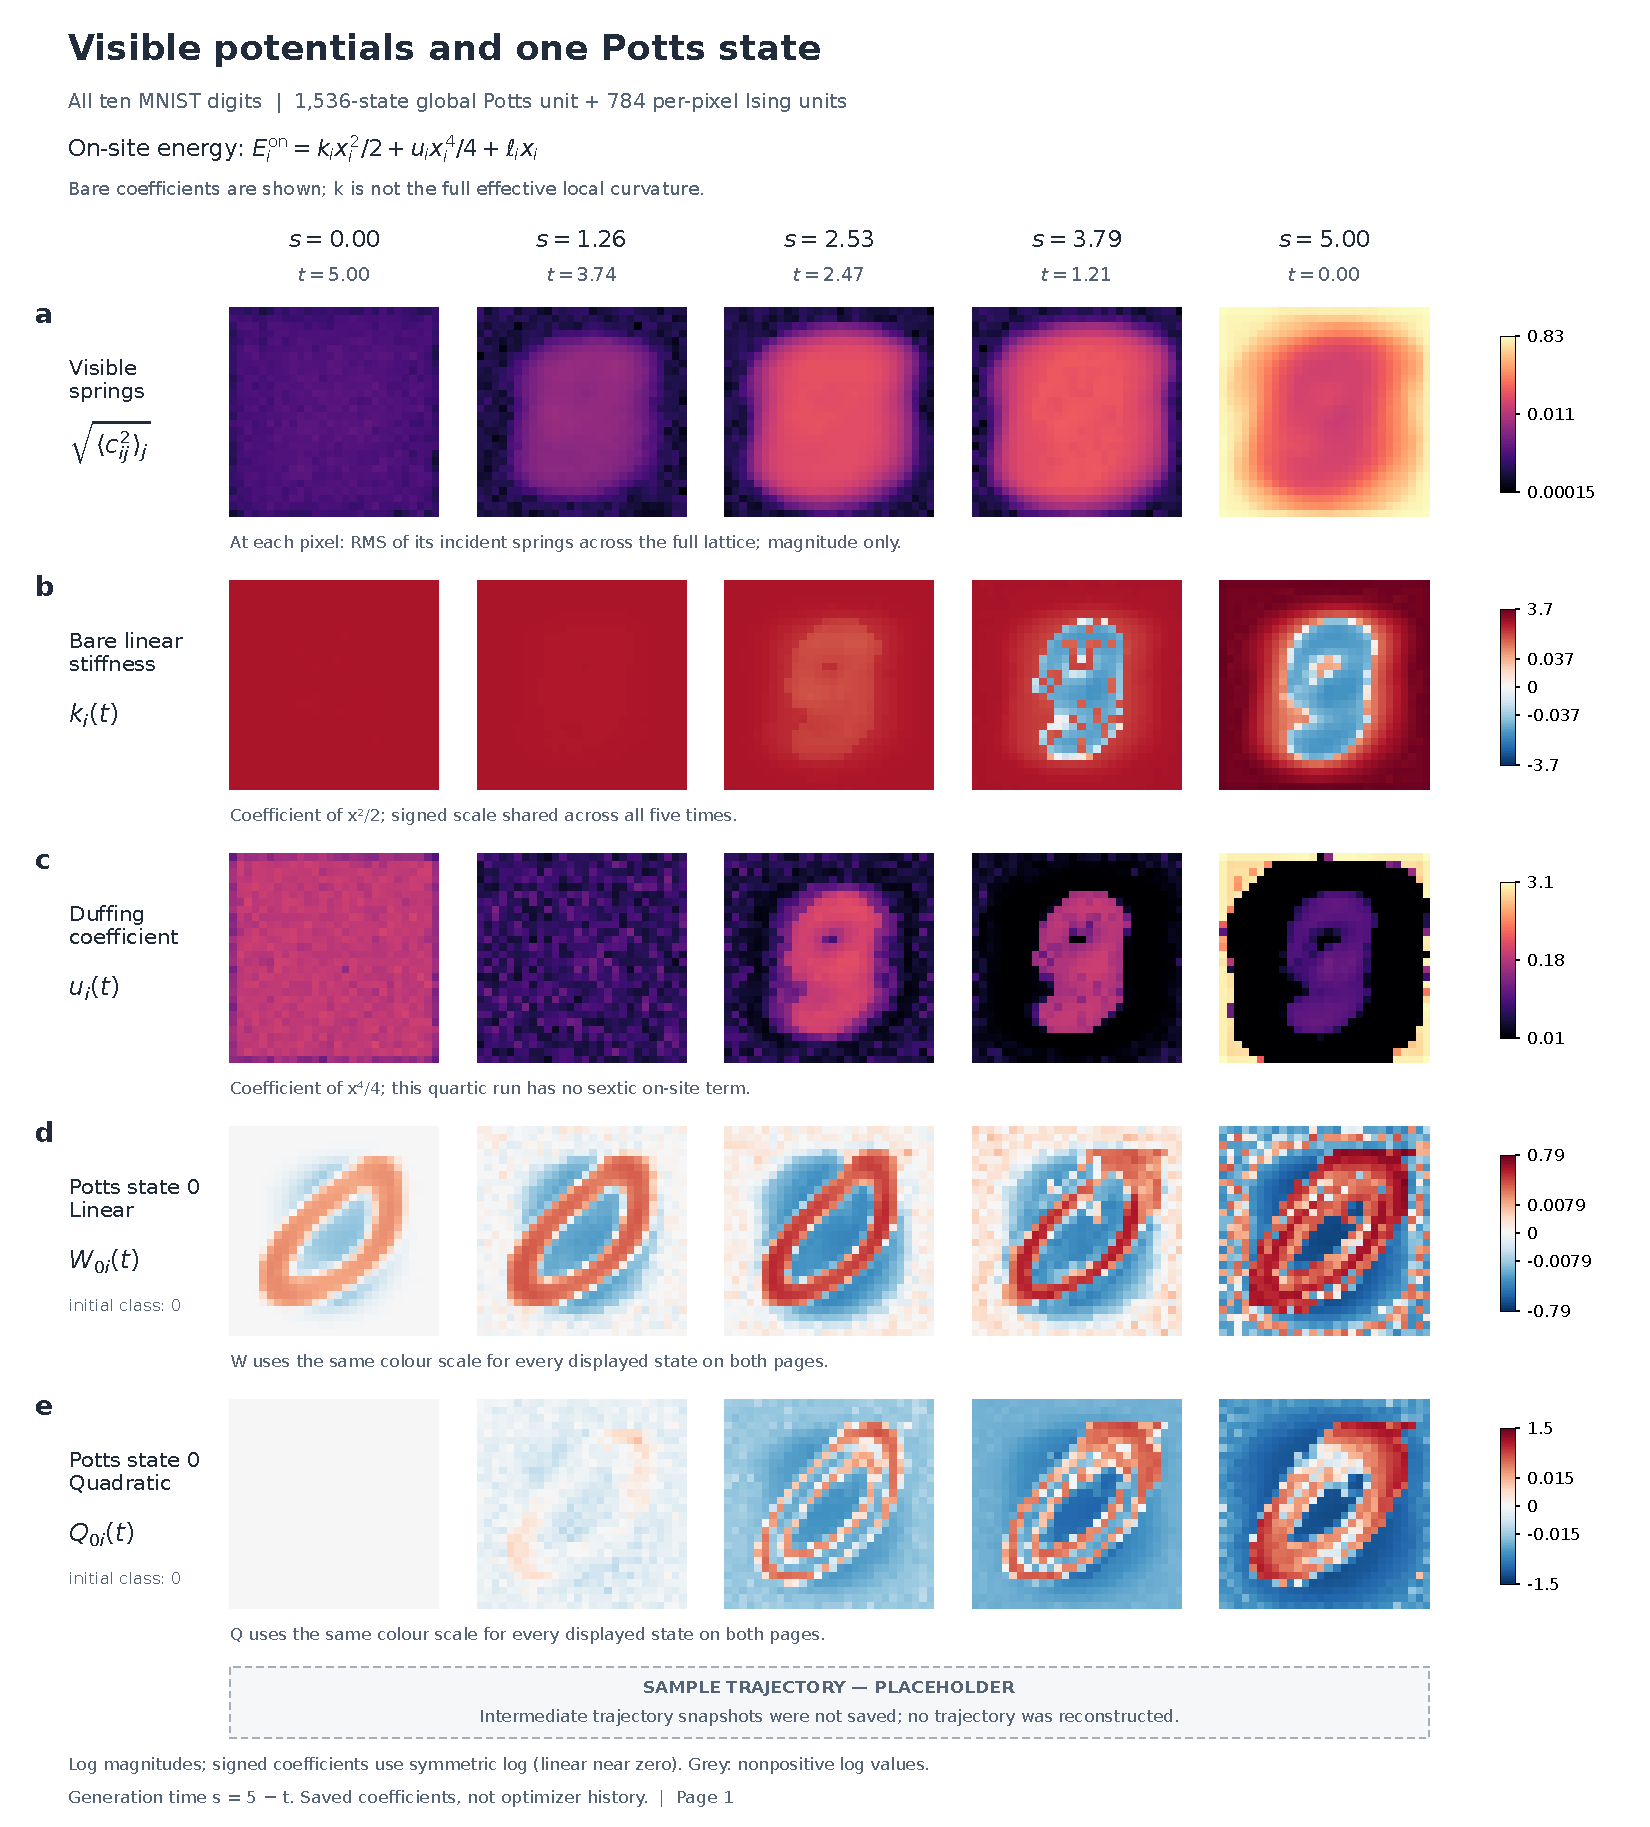
\includegraphics[page=1,width=\textwidth]{figures/parameter_evolution_draft.pdf}
  \caption{\textbf{Parameter evolution and generation of a digit.}
  Saved parameters of the all-ten-digit MNIST model with one global
  1536-state Potts unit and 784 per-pixel Ising units. Columns follow decreasing
  forward diffusion time $t$, from the noisy end to the data end.
  (a) Per-pixel root-mean-square magnitude of incident spring coefficients,
  $\sqrt{d_i^{-1}\sum_{j\in\mathcal{N}(i)}c_{ij}^2}$; $c_{ij}$ multiplies
  $(x_i-x_j)^2$. (b,c) Bare on-site linear stiffness $k_i$ and quartic
  coefficient $u_i$, entering the energy as $k_i x_i^2/2+u_i x_i^4/4$.
  These are bare parameters; hidden couplings also affect the effective curvature.
  (d,e) Linear and quadratic hidden couplings $W_{2i}$ and $Q_{2i}$ for fixed
  Potts state 2 (zero-based index), whose initialization cluster had majority
  digit label 2. This association describes initialization.
  Every parameter row uses the same blue--white--red palette, with its own
  numerical range. Positive spring magnitudes and quartic coefficients use
  logarithmic scales; signed coefficients use symmetric logarithmic scales
  with a linear interval around zero extending to 1\% of the largest absolute
  displayed value. Colours indicate low to high values within each row;
  blue also represents small positive values in (a,c). Limits are fixed across
  times and, for each of $W$ and $Q$, all states on both pages.
  (f) Recorded image evolution under the full trained model at the same times,
  shown in white on black with common pixel-intensity limits $[0,1]$.
  Trajectory 21 of the original 2000-sample base set (seed 2026) was replayed
  and selected visually from final samples 0--99 as an illustrative clear 2.
  Images are recorded states, with no image interpolation. Sampling uses
  conditional mean hidden forces. Other parameters are omitted; displayed
  coefficients retain their raw saved values.}
  \label{fig:parameter_evolution_draft}
\end{figure*}

\begin{figure*}[t]
  \centering
  \includegraphics[page=2,width=\textwidth]{figures/parameter_evolution_draft.pdf}
  \caption{\textbf{Additional fixed Potts states.}
  Linear and quadratic coupling maps for state indices 0, 1 and 4, with the
  same forward times and shared $W$ and $Q$ colour scales as state 2 on the
  preceding page. Their initialization clusters had majority digit labels
  0, 6 and 9, respectively. These labels describe initialization rather than
  measured final-state class purity. Maps retain raw saved coefficients,
  with no common-mode subtraction or per-frame normalization.}
  \label{fig:additional_potts_states_draft}
\end{figure*}

\begin{figure}[t]
  \centering
  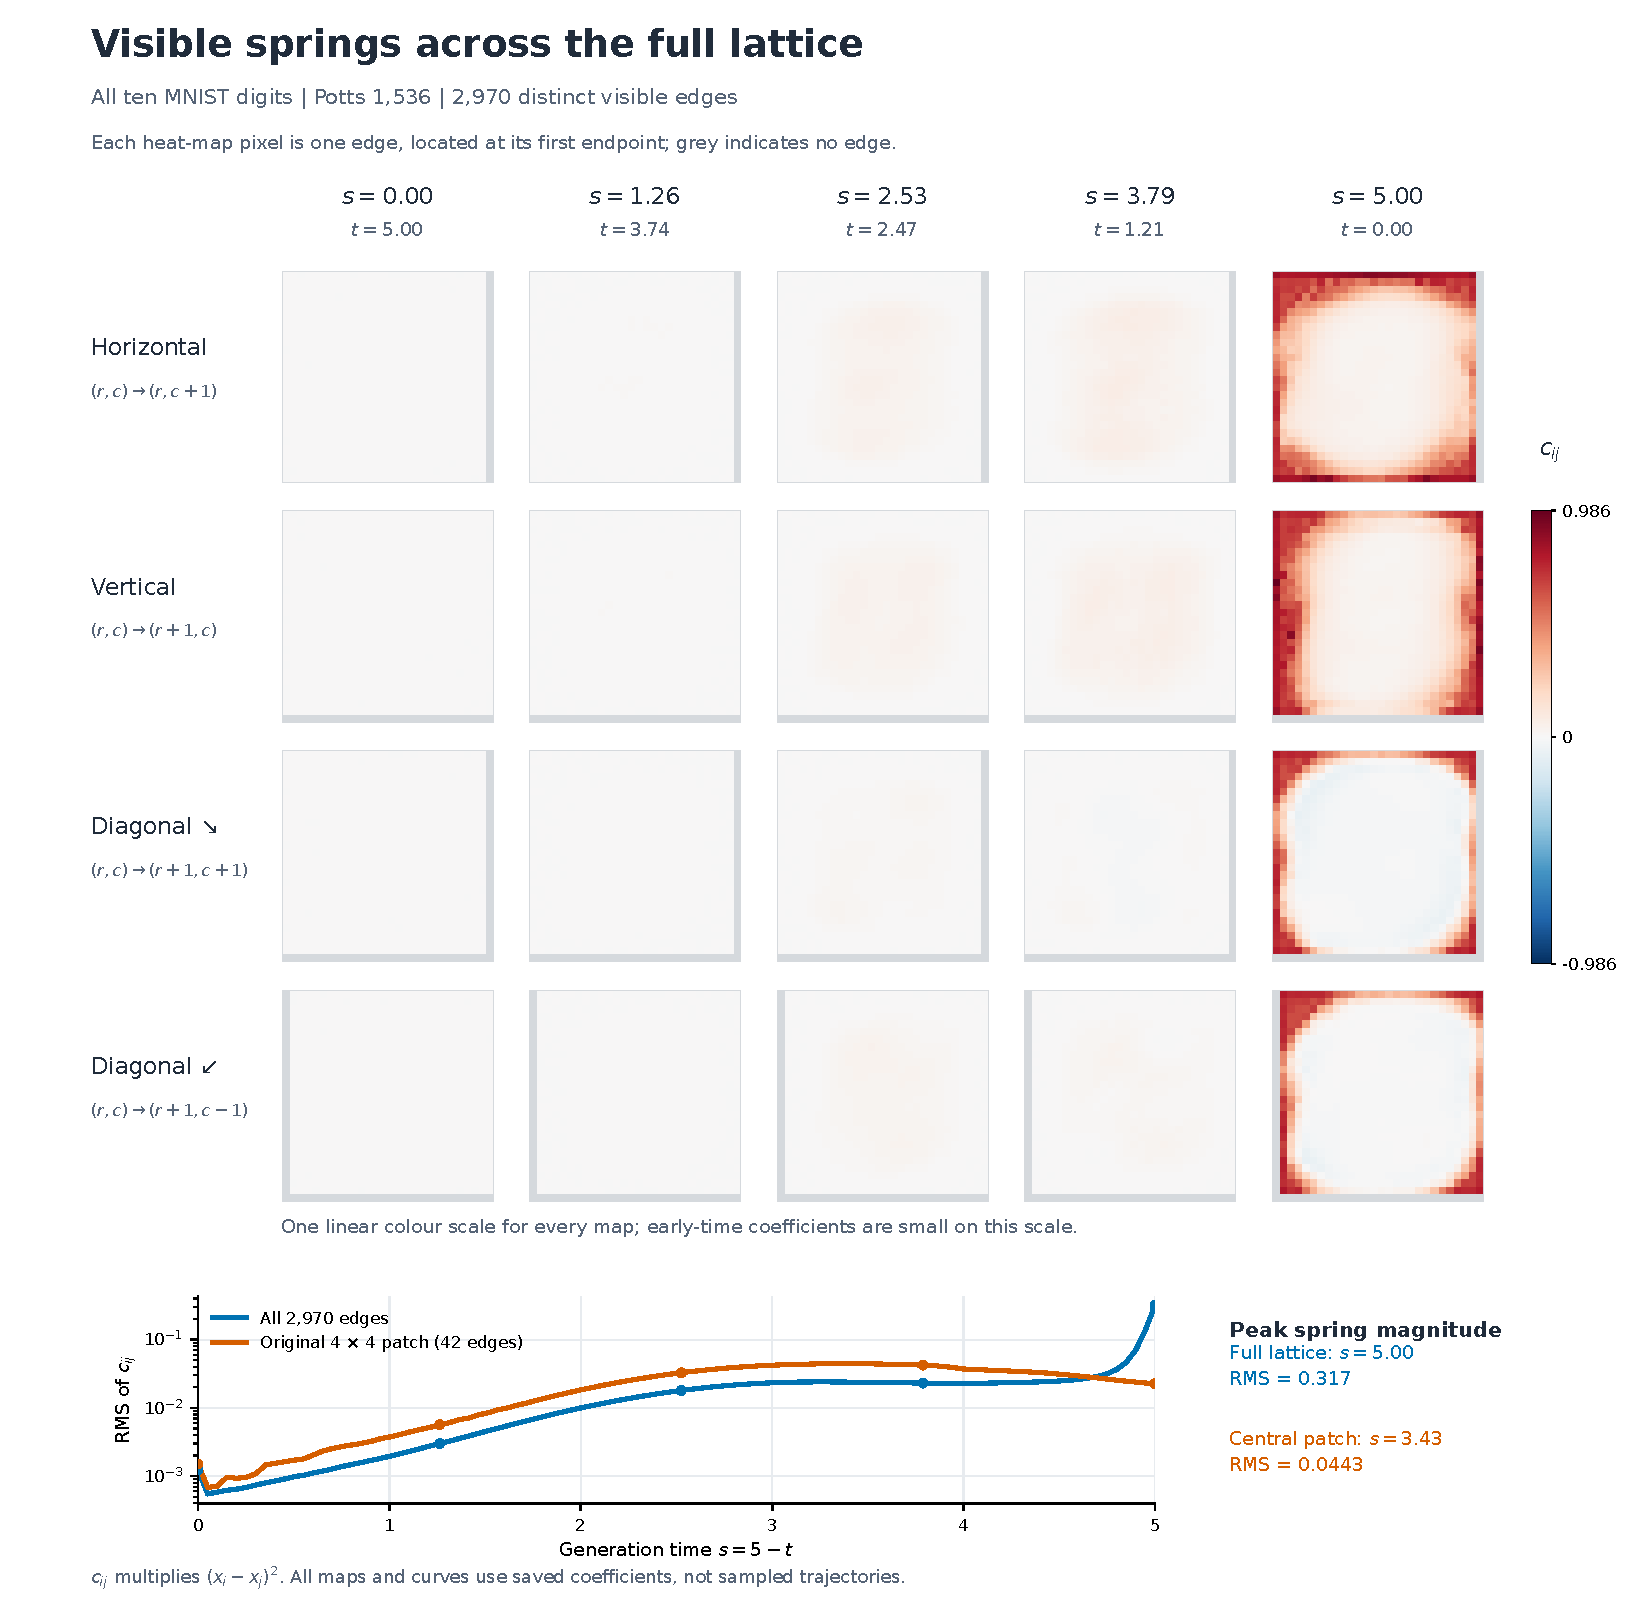
\includegraphics[width=\textwidth]{figures/visible_coupling_evolution.pdf}
  \caption{\textbf{Spatial structure of the visible spring schedule.}
  Signed spring coefficients are separated into horizontal, vertical and two
  diagonal orientations so that each edge appears once. The maps use a common
  colour scale across orientations and displayed times. Strength curves show
  root-mean-square coefficients over all $2970$ edges and over the $42$ edges
  in the central $4\times4$ patch used in the initial graph draft. The
  central patch weakens near the data end, whereas the full-lattice RMS is
  largest at the final time. These are learned coefficient schedules, not
  measurements of trajectory-dependent forces or a controlled explanation
  of the sampling dynamics.}
  \label{fig:visible_coupling_evolution_draft}
\end{figure}

\begin{figure}[t]
  \centering
  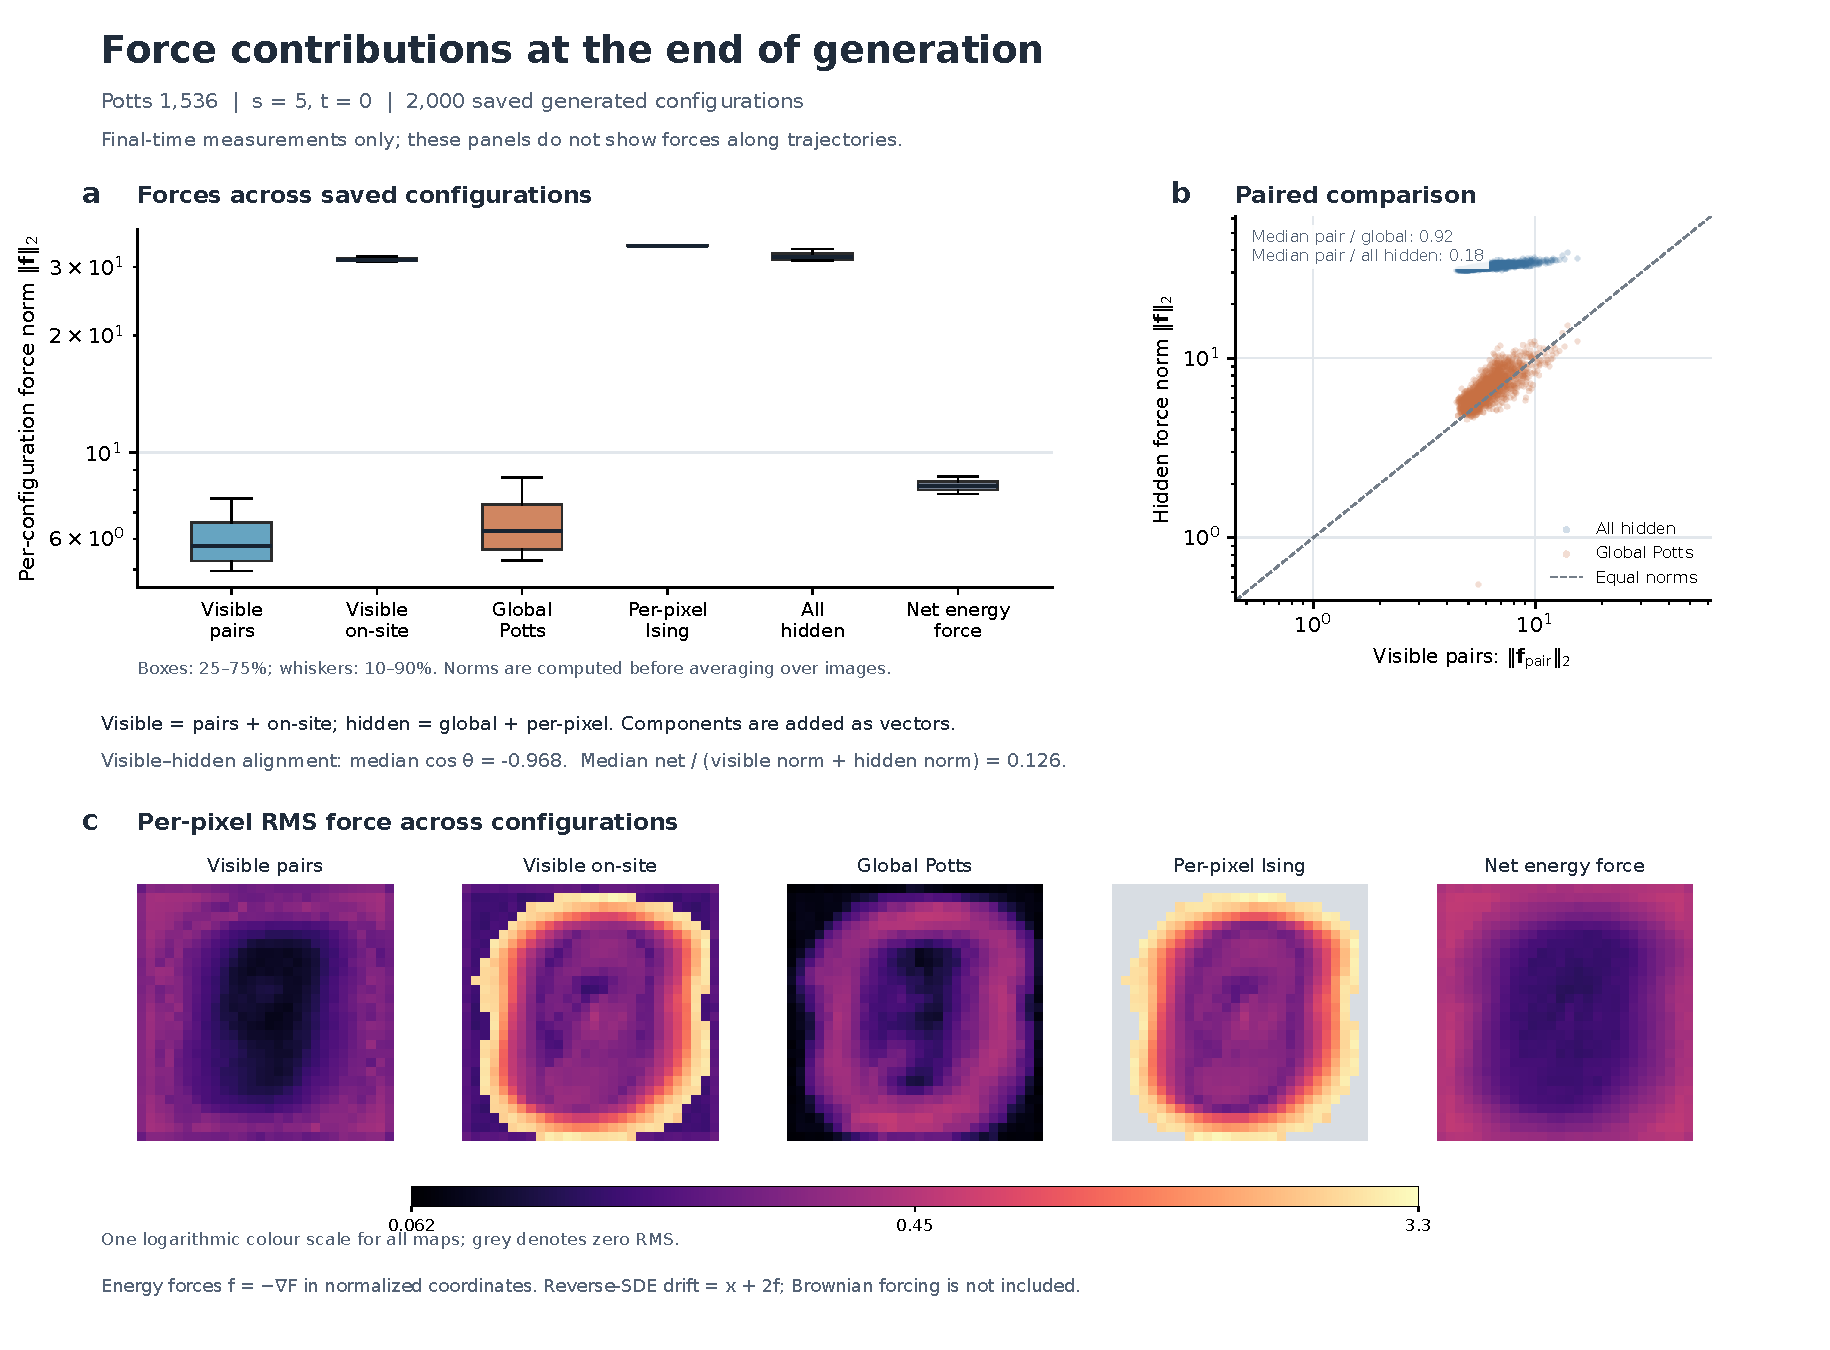
\includegraphics[width=\textwidth]{figures/force_comparison_final.pdf}
  \caption{\textbf{Force contributions at the end of generation.}
  Energy forces evaluated at $t=0$ ($s=5$) on all $2000$ saved generated
  configurations of the Potts1536 model. No configurations were excluded.
  (a) Euclidean norms across the $784$ visible pixels, evaluated separately
  for each configuration, of the visible pair, on-site, global Potts,
  per-pixel Ising, total hidden and net energy forces.
  (b) Paired comparisons against the visible pair-force norm; the diagonal
  indicates equal magnitudes. Hidden contributions are added as vectors
  before calculating the all-hidden norm.
  (c) Per-pixel root-mean-square forces across configurations, using one
  logarithmic colour scale. Alignment and cancellation statistics refer to
  total visible force (pair plus on-site) and total hidden force (global plus
  per-pixel). These are components of $-\nabla F$; the reverse-SDE drift is
  $\mathbf{x}+2(-\nabla F)$. The decomposition describes the saved parameters
  and does not by itself establish causal importance. Intermediate trajectory
  forces are not available from these final configurations.}
  \label{fig:force_comparison_final_draft}
\end{figure}
